%%
%% Automatically generated file from DocOnce source
%% (https://github.com/doconce/doconce/)
%% doconce format html exercises_pandas.do.txt CHAPTER=document BOOK=document APPENDIX=document --latex_todonotes --device=paper --latex_admon_color=1,1,1 --latex_admon=mdfbox -DSOLUTIONS --latex_list_of_exercises=toc --latex_table_format=left --latex_code_style=default:lst[style=blue1]@pypro:lst[style=blue1bar]@dat:lst[style=gray]@sys:vrb[frame=lines,label=\fbox{{\tiny Terminal}},framesep=2.5mm,framerule=0.7pt]

% #define PREAMBLE

% #ifdef PREAMBLE
%-------------------- begin preamble ----------------------

\documentclass[%
twoside,                 % oneside: electronic viewing, twoside: printing
final,                   % draft: marks overfull hboxes, figures with paths
10pt]{article}

\listfiles               %  print all files needed to compile this document

\usepackage{relsize,makeidx,color,setspace,amsmath,amsfonts,amssymb}
\usepackage[table]{xcolor}
\usepackage{bm,ltablex,microtype}

\usepackage[pdftex]{graphicx}

% Packages for typesetting blocks of computer code
\usepackage{fancyvrb,framed,moreverb}

% Define colors
\definecolor{orange}{cmyk}{0,0.4,0.8,0.2}
\definecolor{tucorange}{rgb}{1.0,0.64,0}
\definecolor{darkorange}{rgb}{.71,0.21,0.01}
\definecolor{darkgreen}{rgb}{.12,.54,.11}
\definecolor{myteal}{rgb}{.26, .44, .56}
\definecolor{gray}{gray}{0.45}
\definecolor{mediumgray}{gray}{.8}
\definecolor{lightgray}{gray}{.95}
\definecolor{brown}{rgb}{0.54,0.27,0.07}
\definecolor{purple}{rgb}{0.5,0.0,0.5}
\definecolor{darkgray}{gray}{0.25}
\definecolor{darkblue}{rgb}{0,0.08,0.45}
\definecolor{darkblue2}{rgb}{0,0,0.8}
\definecolor{lightred}{rgb}{1.0,0.39,0.28}
\definecolor{lightgreen}{rgb}{0.48,0.99,0.0}
\definecolor{lightblue}{rgb}{0.53,0.81,0.92}
\definecolor{lightblue2}{rgb}{0.3,0.3,1.0}
\definecolor{lightpurple}{rgb}{0.87,0.63,0.87}
\definecolor{lightcyan}{rgb}{0.5,1.0,0.83}

\colorlet{comment_green}{green!50!black}
\colorlet{string_red}{red!60!black}
\colorlet{keyword_pink}{magenta!70!black}
\colorlet{indendifier_green}{green!70!white}

% Backgrounds for code
\definecolor{cbg_gray}{rgb}{.95, .95, .95}
\definecolor{bar_gray}{rgb}{.92, .92, .92}

\definecolor{cbg_yellowgray}{rgb}{.95, .95, .85}
\definecolor{bar_yellowgray}{rgb}{.95, .95, .65}

\colorlet{cbg_yellow2}{yellow!10}
\colorlet{bar_yellow2}{yellow!20}

\definecolor{cbg_yellow1}{rgb}{.98, .98, 0.8}
\definecolor{bar_yellow1}{rgb}{.98, .98, 0.4}

\definecolor{cbg_red1}{rgb}{1, 0.85, 0.85}
\definecolor{bar_red1}{rgb}{1, 0.75, 0.85}

\definecolor{cbg_blue1}{rgb}{0.87843, 0.95686, 1.0}
\definecolor{bar_blue1}{rgb}{0.7,     0.95686, 1}

\usepackage{listingsutf8}

% Common lstlisting parameters

\usepackage{calc}
\newlength{\lstboxwidth}  % width of lst box
\newlength{\framethickness}
\setlength{\framethickness}{0.5mm}
% for frame=trbl and a framerule that has significant size, set
% xleftmargin=5mm and xrightmargin=5mm.

\lstset{
  basicstyle=\small \ttfamily,
  breaklines=false,          % break/wrap lines
  breakatwhitespace=true,    % let linebreaks happen at whitespace
  breakindent=40pt,
  tab=,
  tabsize=4,                 % tab means 4 spaces
  %belowskip=\smallskipamount,  % space between code and text below
  xleftmargin=2mm,           % indentation of code frame
  xrightmargin=0mm,
  framexleftmargin=2mm,      % add frame space to the left of the code box
  %numbers=left,             % put line numbers on the left
  %stepnumber=2,             % stepnumber=1 numbers each line, =n every n lines
  framerule=\framethickness, % thickness of frame
  aboveskip=2ex,             % vertical space above code frame
  showstringspaces=false,    % show spaces in strings with an underscore
  showspaces=false,          % show spaces with an underscore
  showtabs=false,
  keepspaces=true,
  columns=fullflexible,      % tighter character kerning, like verb
  escapeinside={(*@}{@*)},   % (*@ \pause @*) in slides and math in code blocks
  extendedchars=\true,       % allows non-ascii chars, does not work with utf-8
}

% Internally defined styles for lstlisting

% Use this one without additional background color
\lstdefinestyle{blue1}{              % blue1 background for code snippets
backgroundcolor=\color{cbg_blue1},
}

% Use this one without additional background color
% (same as blue1, but with bar_blue1 frame)
\lstdefinestyle{blue1bar}{           % blue1 background for complete programs
backgroundcolor=\color{cbg_blue1},
frame=tb,                            % include frame
rulecolor=\color{bar_blue1},         % frame color
}

% Use this one without additional background color
\lstdefinestyle{gray}{
backgroundcolor=\color{cbg_gray},
%frame=tb,                            % include frame
%framerule=0.4pt                      % thickness of frame
rulecolor=\color{black!40},           % frame color
}

\lstdefinestyle{simple}{
commentstyle={},
}

% end of custom lstdefinestyles

\usepackage[T1]{fontenc}
%\usepackage[latin1]{inputenc}
\usepackage{ucs}
\usepackage[utf8x]{inputenc}

\usepackage{lmodern}         % Latin Modern fonts derived from Computer Modern

% Hyperlinks in PDF:

\usepackage{hyperref}
\hypersetup{
    breaklinks=true,
    colorlinks=true,
    linkcolor=black,
    urlcolor=black,
    citecolor=black,
    filecolor=black,
    %filecolor=blue,
    pdfmenubar=true,
    pdftoolbar=true,
    bookmarksdepth=3   % Uncomment (and tweak) for PDF bookmarks with more levels than the TOC
    }
%\hyperbaseurl{}   % hyperlinks are relative to this root

\setcounter{tocdepth}{2}  % levels in table of contents

% Tricks for having figures close to where they are defined:
% 1. define less restrictive rules for where to put figures
\setcounter{topnumber}{2}
\setcounter{bottomnumber}{2}
\setcounter{totalnumber}{4}
\renewcommand{\topfraction}{0.95}
\renewcommand{\bottomfraction}{0.95}
\renewcommand{\textfraction}{0}
\renewcommand{\floatpagefraction}{0.75}
% floatpagefraction must always be less than topfraction!
% 2. ensure all figures are flushed before next section
\usepackage[section]{placeins}
% 3. enable begin{figure}[H] (often leads to ugly pagebreaks)
%\usepackage{float}\restylefloat{figure}

\usepackage[framemethod=TikZ]{mdframed}

% --- begin definitions of admonition environments ---

% Admonition style "mdfbox" is an oval colored box based on mdframed
% "notice" admon
\definecolor{mdfbox_notice_background}{rgb}{1,1,1}
\newmdenv[
  skipabove=15pt,
  skipbelow=15pt,
  outerlinewidth=0,
  backgroundcolor=mdfbox_notice_background,
  linecolor=black,
  linewidth=2pt,       % frame thickness
  frametitlebackgroundcolor=mdfbox_notice_background,
  frametitlerule=true,
  frametitlefont=\normalfont\bfseries,
  shadow=false,        % frame shadow?
  shadowsize=11pt,
  leftmargin=0,
  rightmargin=0,
  roundcorner=5,
  needspace=0pt,
]{notice_mdfboxmdframed}

\newenvironment{notice_mdfboxadmon}[1][]{
\begin{notice_mdfboxmdframed}[frametitle=#1]
}
{
\end{notice_mdfboxmdframed}
}

% Admonition style "mdfbox" is an oval colored box based on mdframed
% "summary" admon
\definecolor{mdfbox_summary_background}{rgb}{1,1,1}
\newmdenv[
  skipabove=15pt,
  skipbelow=15pt,
  outerlinewidth=0,
  backgroundcolor=mdfbox_summary_background,
  linecolor=black,
  linewidth=2pt,       % frame thickness
  frametitlebackgroundcolor=mdfbox_summary_background,
  frametitlerule=true,
  frametitlefont=\normalfont\bfseries,
  shadow=false,        % frame shadow?
  shadowsize=11pt,
  leftmargin=0,
  rightmargin=0,
  roundcorner=5,
  needspace=0pt,
]{summary_mdfboxmdframed}

\newenvironment{summary_mdfboxadmon}[1][]{
\begin{summary_mdfboxmdframed}[frametitle=#1]
}
{
\end{summary_mdfboxmdframed}
}

% Admonition style "mdfbox" is an oval colored box based on mdframed
% "warning" admon
\definecolor{mdfbox_warning_background}{rgb}{1,1,1}
\newmdenv[
  skipabove=15pt,
  skipbelow=15pt,
  outerlinewidth=0,
  backgroundcolor=mdfbox_warning_background,
  linecolor=black,
  linewidth=2pt,       % frame thickness
  frametitlebackgroundcolor=mdfbox_warning_background,
  frametitlerule=true,
  frametitlefont=\normalfont\bfseries,
  shadow=false,        % frame shadow?
  shadowsize=11pt,
  leftmargin=0,
  rightmargin=0,
  roundcorner=5,
  needspace=0pt,
]{warning_mdfboxmdframed}

\newenvironment{warning_mdfboxadmon}[1][]{
\begin{warning_mdfboxmdframed}[frametitle=#1]
}
{
\end{warning_mdfboxmdframed}
}

% Admonition style "mdfbox" is an oval colored box based on mdframed
% "question" admon
\definecolor{mdfbox_question_background}{rgb}{1,1,1}
\newmdenv[
  skipabove=15pt,
  skipbelow=15pt,
  outerlinewidth=0,
  backgroundcolor=mdfbox_question_background,
  linecolor=black,
  linewidth=2pt,       % frame thickness
  frametitlebackgroundcolor=mdfbox_question_background,
  frametitlerule=true,
  frametitlefont=\normalfont\bfseries,
  shadow=false,        % frame shadow?
  shadowsize=11pt,
  leftmargin=0,
  rightmargin=0,
  roundcorner=5,
  needspace=0pt,
]{question_mdfboxmdframed}

\newenvironment{question_mdfboxadmon}[1][]{
\begin{question_mdfboxmdframed}[frametitle=#1]
}
{
\end{question_mdfboxmdframed}
}

% Admonition style "mdfbox" is an oval colored box based on mdframed
% "block" admon
\definecolor{mdfbox_block_background}{rgb}{1,1,1}
\newmdenv[
  skipabove=15pt,
  skipbelow=15pt,
  outerlinewidth=0,
  backgroundcolor=mdfbox_block_background,
  linecolor=black,
  linewidth=2pt,       % frame thickness
  frametitlebackgroundcolor=mdfbox_block_background,
  frametitlerule=true,
  frametitlefont=\normalfont\bfseries,
  shadow=false,        % frame shadow?
  shadowsize=11pt,
  leftmargin=0,
  rightmargin=0,
  roundcorner=5,
  needspace=0pt,
]{block_mdfboxmdframed}

\newenvironment{block_mdfboxadmon}[1][]{
\begin{block_mdfboxmdframed}[frametitle=#1]
}
{
\end{block_mdfboxmdframed}
}

% --- end of definitions of admonition environments ---

% prevent orhpans and widows
\clubpenalty = 10000
\widowpenalty = 10000

% --- end of standard preamble for documents ---


% insert custom LaTeX commands...

\raggedbottom
\makeindex
\usepackage[totoc]{idxlayout}   % for index in the toc
\usepackage[nottoc]{tocbibind}  % for references/bibliography in the toc

%-------------------- end preamble ----------------------

\begin{document}

% matching end for #ifdef PREAMBLE
% #endif

\newcommand{\exercisesection}[1]{\subsection*{#1}}

% This file is to be run by preprocess to produce newcommands.tex
% to be included in .tex files.
% There are format-specific tests here for the newcommands (i.e.,
% different definitions of the commands depending on latex or mathjax).

% Newcommands for LaTeX math.
\newcommand{\no}{\nonumber}
\newcommand{\tp}{\thinspace .}
\renewcommand{\Re}{\bbbr}
\newcommand{\Oof}[1]{\mathcal{O}(#1)}
\newcommand{\Prob}[1]{\hbox{P}(#1)}
\newcommand{\Var}[1]{\hbox{Var}(#1)}
\newcommand{\Cov}[2]{\hbox{Cov}(#1,#2)}
\newcommand{\StDev}[1]{\hbox{StDev}(#1)}
\newcommand{\co}{CO$_2$}

% Use footnotesize in subscripts
\newcommand{\subsc}[2]{#1_{\mbox{\footnotesize #2}}}




% ------------------- main content ----------------------



% ----------------- title -------------------------

\thispagestyle{empty}

\begin{center}
{\LARGE\bf
\begin{spacing}{1.25}
Pandas gym
\end{spacing}
}
\end{center}

% ----------------- author(s) -------------------------

\begin{center}
{\bf Prepared as part of Python for Subsurface Applications and Management${}^{}$} \\ [0mm]
\end{center}


\begin{center}
{\bf Aksel Hiorth University of Stavanger${}^{}$} \\ [0mm]
\end{center}

\begin{center}
% List of all institutions:
\end{center}
    
% ----------------- end author(s) -------------------------

% --- begin date ---
\begin{center}
Mar 26, 2023
\end{center}
% --- end date ---

\vspace{1cm}


\paragraph{Learning objectives:}

\begin{enumerate}
\item how to create a DataFrame

\item plot data in DataFrame

\item write code that is robust, i.e.~gives error messages when it fails

\item do simple statistics on data in a DataFrame

\item group and filter data

\item work with files and folders, split data into different files
\end{enumerate}

\noindent
\section{Exercise 1 Create a data frame}
In the folder \texttt{data} there is a file named \Verb!field_production_monthly.csv!.

\begin{enumerate}
\item Read this file into a Pandas DataFrame

\item Make a function that reads a file into a DataFrame, and returns an error message if it fails to open the file
\end{enumerate}

\noindent





\begin{lstlisting}[language=Python,style=blue1bar]
df = pd.read_csv(..)

def read_data_frame(file_name,sep=','):
 ... write function

\end{lstlisting}


\paragraph{SOLUTION:}

If the csv file is located in the same folder as your python program


\begin{lstlisting}[language=Python,style=blue1bar]
df=pd.read_csv('../data/field_production_monthly.csv', sep=',')

\end{lstlisting}

Next, we make a function











\begin{lstlisting}[language=Python,style=blue1bar]
def read_data_frame(file_name,sep=','):
    try:
        df=pd.read_csv(file_name,sep=sep)
        return df
    except:
        print('Could not open file: ', file_name)
        return pd.DataFrame()

df=read_data_frame('../data/field_production_monthly.csv')

\end{lstlisting}


There are a couple of things to note here, first it is the try except statement. This basically tells Python to try to execute the \Verb!pd.read_csv()! command, if this fail it jumps to the except statement and execute that. This is an extremely elegant way to make your code able to run without stopping and also write out your own error messages instead of the usual error messages generated from Python. Next, it is a good practice to return an object of the same type, thus here we returns an empty DataFrame. Note that in the function we have also used \texttt{sep=','} as the default argument. 

\section{Exercise 2 Extract data for Snorre}
The file \Verb!field_production_gross_monthly.csv! contains production data from the Norwegian Petroleum Directorate \href{{https://factpages.npd.no/}}{factpages}\footnote{\texttt{https://factpages.npd.no/}}.

\begin{enumerate}
\item Extract a DataFrame for the Snorre field

\item Plot the production of oil equivalents as a function of time
\begin{itemize}

  \item Use Matplotlib, and

  \item the built in plotting functionality of Pandas

\end{itemize}

\noindent
\item Compare your plot with the one on the \href{{https://factpages.npd.no/en/field/PageView/All/43718}}{factpages}\footnote{\texttt{https://factpages.npd.no/en/field/PageView/All/43718}}. Use the \href{{https://pandas.pydata.org/docs/reference/api/pandas.DataFrame.groupby.html}}{\nolinkurl{pd.groupby()}\footnote{\texttt{https://pandas.pydata.org/docs/reference/api/pandas.DataFrame.groupby.html}}} function to make a new data frame that contains the production per year and see if you can reproduce figure~\ref{fig:snorre} from the factpages.
\end{enumerate}

\noindent
\begin{figure}[!ht]  % fig:snorre
  \centerline{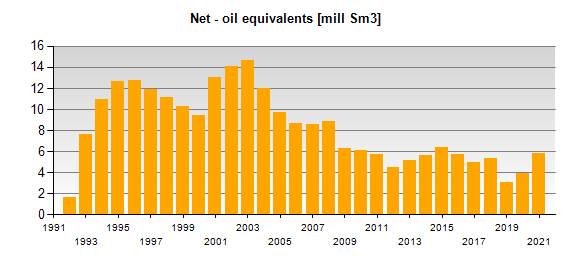
\includegraphics[width=1.0\linewidth]{fig-pandas/snorre.png}}
  \caption{
  Yearly production from the Snorre field. \label{fig:snorre}
  }
\end{figure}
%\clearpage % flush figures fig:snorre



\begin{lstlisting}[language=Python,style=blue1bar]
# fill inn code

\end{lstlisting}


\section{Exercise 3 Extract data for any field}
Now we want to write some functions that are more general, which can extract information from any field.
\begin{enumerate}
\item Make a general function that can extract a DataFrame given any name of a field in the database. If you want to be fancy you could also make the function case insensitive. The function should write a reasonable error message if something went wrong

\item Write a function that takes as argument a DataFrame for a given field and makes a plot of the monthly production of oil equivalents. Give the plot a reasonable title and axes labels
\end{enumerate}

\noindent










\begin{lstlisting}[language=Python,style=blue1bar]
df_full=pd.read_csv('../data/field_production_monthly.csv',sep=',')

def get_field_data_frame(field_name,df=df_full):
    '''
    Returns a dataframe given a field name, 
    returns empty dataframe if field does not exist 
    '''
    #... fill in code 
    

\end{lstlisting}

\paragraph{SOLUTION:}



























\begin{lstlisting}[language=Python,style=blue1bar]
df_full=pd.read_csv('../data/field_production_monthly.csv',sep=',')

def get_field_data_frame(field_name,df=df_full):
    '''
    Returns a dataframe given a field name, 
    returns empty dataframe if field does not exist 
    '''
    FIELD_NAME=field_name.upper()
    all_fields=df['prfInformationCarrier'].unique()
    if FIELD_NAME in all_fields:
        return df[df['prfInformationCarrier']==FIELD_NAME]
    else:
        print('Field name ', field_name, ' does not exists')
        print('Available field names are: ')
        print(all_fields)
        return pd.DataFrame()
df=get_field_data_frame('snore') # Wrong name
df=get_field_data_frame('snorRe')

def plot_field_prod_data(df,y='prfPrdOeNetMillSm3'):
    name=df['prfInformationCarrier'].iloc[0] 
    df['time']=df['prfYear']+df['prfMonth']/12
    df.plot(x='time',y=y,title=name,grid=True,xlabel='Years',ylabel=r'Production per month [mill Sm$^3$]')

plot_field_prod_data(df)

\end{lstlisting}

If you are having problem understanding the code above, you should set \Verb!df=df_full!, and \Verb!field_name='snorre!, and then execute each line in a jupyter notebook. Note that we send in the full DataFrame to the function, this is important if the database is large, you do not want read the excel or csv file over and over each time you call the function - this significantly slows down your code!

\section{Exercise 4 Plot the total production data for NCS}
\begin{enumerate}
\item Use the \href{{https://pandas.pydata.org/docs/reference/api/pandas.DataFrame.groupby.html}}{\nolinkurl{pd.groupby()}\footnote{\texttt{https://pandas.pydata.org/docs/reference/api/pandas.DataFrame.groupby.html}}}  functionality in Pandas to create a DataFrame containing production data for NCS as a whole

\item Make a plot of the production
\end{enumerate}

\noindent
\paragraph{SOLUTION:}









\begin{lstlisting}[language=Python,style=blue1bar]
# create data frame
df_ncs=df_full.groupby('prfYear').sum()

# plot the data
df_ncs.plot(y=df_full.columns[3:9],grid=True)
# alternatively
df_ncs.plot(y=df_full.columns[3:9],grid=True,subplots=True)

\end{lstlisting}


\section{Exercise 5 Split data into folders and files}

Create a new data directory in which you create one folder for each field that contains an excel sheet with production data for that field. Use the \texttt{Pathlib} library to create directories.


\begin{notice_mdfboxadmon}[Special characters in names.]
Here you will encounter names with special characters, it is usually a good idea to replace those characters with a suitable replacement, before creating names or directories. To help you, you can use the function \Verb!replace_chars! below.
\end{notice_mdfboxadmon} % title: Special characters in names.












\begin{lstlisting}[language=Python,style=blue1bar]
# fill in code
from pathlib import Path
def replace_chars(name, chars=["/"," ", "Å", "Ø", "Æ"], new_chars=["_","_","AA","O","AE"]):
    ''' replace Norwegian characters, space and slash in names'''
    new_name = name
    for ch,nch in zip(chars,new_chars):
        new_name = new_name.replace(ch, nch)
    return new_name


\end{lstlisting}


\paragraph{SOLUTION:}














\begin{lstlisting}[language=Python,style=blue1bar]
from pathlib import Path
col='prfInformationCarrier'
fields = df_full[col].unique() #skip duplicates
data_folder=Path('../production-data')
data_folder.mkdir(exist_ok=True)
for field in fields:
    new_name=replace_chars(field)
    new_path=data_folder / new_name
    new_path.mkdir(exist_ok=True)
    excel_file=new_name+'.xlsx'
    df2=df_full[df_full[col]==field]
    df2.to_excel(new_path/excel_file,index=False)

\end{lstlisting}


\section{Exercise 6 Combine DataFrames}
Write a code to collect all the excel files you stored in different folder into a single DataFrame (Hint: use \href{{https://pandas.pydata.org/docs/reference/api/pandas.concat.html}}{\nolinkurl{concat()}\footnote{\texttt{https://pandas.pydata.org/docs/reference/api/pandas.concat.html}}} to combine data)



\begin{lstlisting}[language=Python,style=blue1bar]
df_new=pd.DataFrame()

\end{lstlisting}


\paragraph{SOLUTION:}













\begin{lstlisting}[language=Python,style=blue1bar]
df_new=pd.DataFrame()
data_folder=Path('../production-data')
for dir in data_folder.iterdir():
    if dir.is_dir():      
        file=dir.name+'.xlsx'
        try:
            df=pd.read_excel(dir/file)
            print('Reading file ', file)
            df_new=pd.concat([df_new,df],ignore_index=True)
        except:
            print('No data in folder ', dir.name)

\end{lstlisting}


\section{Exercise 7 Scrap data from the web}
In this exercise we will collect data from the web, note that this will require some additional checking if the data you have read is of the correct type. Note that you can always do \texttt{df.dtypes} to list the types in the DataFrame.

\begin{enumerate}
\item Use the function \href{{https://pandas.pydata.org/docs/reference/api/pandas.read_html.html}}{\nolinkurl{pandas.read_html()}\footnote{\texttt{https://pandas.pydata.org/docs/reference/api/pandas.read\_html.html}}} to scrap production data from the Snorre field directly from \href{{https://factpages.npd.no/en/field/PageView/All/43718}}{the NPD factpages}\footnote{\texttt{https://factpages.npd.no/en/field/PageView/All/43718}}. (Hint: \Verb!pandas.read_html()! returns a list containing all tables in a website as DataFrames)

\item Make a plot of the production data and compare with the production data in figure~\ref{fig:snorre}. (Hint: you might need to sort values in the DataFrame and to convert some values to the correct type)
\end{enumerate}

\noindent


\begin{lstlisting}[language=Python,style=blue1bar]
# enter code here

\end{lstlisting}


\paragraph{SOLUTION:}




\begin{lstlisting}[language=Python,style=blue1bar]
df_lists=pd.read_html('https://factpages.npd.no/en/field/PageView/All/43718')
df_prod=df_lists[14] # production data are in table no 14

\end{lstlisting}


Next, we need to drop the first column




\begin{lstlisting}[language=Python,style=blue1bar]
df_prod2=df_prod.drop([0])
print(df_prod2)
print(df_prod2.dtypes)

\end{lstlisting}


There are two challenges (at least when I did this) 1) One column has been named \texttt{Unnamed: 0}, this is the column with the year data 2) the year data are read in as string (or \texttt{dtype: object}) and we need to convert to integer or float



\begin{lstlisting}[language=Python,style=blue1bar]
df_prod2=df_prod2.rename(columns={df_prod2.columns[0]:"Year"})
df_prod2['Year']=pd.to_numeric(df_prod2['Year'])

\end{lstlisting}

Next, we need to sort the data if we want to plot them in historical correct order




\begin{lstlisting}[language=Python,style=blue1bar]
df_prod2=df_prod2.set_index("Year")
df_prod2=df_prod2.sort_index()
df_prod2

\end{lstlisting}

Finally, we can do the plotting



\begin{lstlisting}[language=Python,style=blue1bar]
df_prod2.plot(y=df_prod2.columns[1:],grid=True)
df_prod2.plot.bar(y=df_prod2.columns[-1])

\end{lstlisting}


% ------------------- end of main content ---------------

% #ifdef PREAMBLE
\end{document}
% #endif

